\documentclass[12pt]{article}

% --- Estilo base del usuario ---
\usepackage{setspace}
\usepackage{newtxtext,newtxmath}
\setstretch{1.5}

\usepackage{amsmath}
\usepackage[utf8]{inputenc}
\usepackage[spanish]{babel}
\usepackage[letterpaper, left=3cm, right=2.5cm, top=2.5cm, bottom=2.5cm]{geometry}

\usepackage{graphicx}
\usepackage{titlesec}
\usepackage{lipsum}
\usepackage{pdfpages}
\usepackage{comment}
\usepackage{float}
\usepackage{enumitem}
\graphicspath{{./Imagenes/}}

\usepackage{pdfpages}


\usepackage{siunitx}

\sisetup{
	output-decimal-marker = {,}, % imprime coma decimal
	group-separator       = {.}, % separador de miles
	group-minimum-digits  = 4,   % agrupar a partir de 4 dígitos (opcional)
	% opcional: aceptar tanto punto como coma en la entrada
	input-decimal-markers = {.,,}
}


%----Empezar cada section enuna hoja nueva 
\let\oldsection\section
\renewcommand{\section}{\clearpage\oldsection}


% --- Encabezado: número SOLO arriba derecha ---
\usepackage{fancyhdr}
\pagestyle{fancy}
\fancyhf{}
\fancyhead[R]{\thepage}
\renewcommand{\headrulewidth}{0pt}
\fancypagestyle{plain}{%
	\fancyhf{}
	\fancyhead[R]{\thepage}
	\renewcommand{\headrulewidth}{0pt}
}

% --- Tabla de contenido con líneas punteadas ---
\usepackage{tocloft}
\renewcommand{\cftsecleader}{\cftdotfill{\cftdotsep}}
\renewcommand{\cftdotsep}{1.5}
\renewcommand{\contentsname}{Contenido} % título del \tableofcontents


% --- Hipervínculos clicables en el índice (cargar casi al final) ---
\usepackage[hidelinks]{hyperref}
% Si prefieres verlos en color:
% \hypersetup{colorlinks=true, linkcolor=blue}

% Listas
\setlist[enumerate]{listparindent=\parindent, parsep=0pt}

\begin{document}
	
	% ===== ÍNDICE (no numera ni cuenta) =====
	\section*{Contenido} % título visible (no entra al TOC)
	\tableofcontents
	\thispagestyle{empty} % sin número en esta(s) página(s)
	\clearpage
	% Reiniciar para que "Objetivos" sea página 1
	\pagenumbering{arabic}
	\setcounter{page}{1}
	
	% ===== CONTENIDO =====
	\section{Objetivos}
	
	\subsection{Objetivo general}
	Realizar las prácticas profesionales en la empresa \textit{Construcción e Ingeniería S.A.}, aplicando los conocimientos teóricos y prácticos de Ingeniería Civil con énfasis en topografía, a través de la ejecución de levantamientos, replanteos y control de niveles que contribuyan al desarrollo y al aseguramiento de la calidad de las obras.
	
	\subsection{Objetivos específicos}
	\begin{itemize}
		\item Ejecutar y apoyar en levantamientos topográficos utilizando equipos e instrumentos adecuados para la obtención precisa de datos del terreno.
		\item Participar en el trazado y control de obras civiles, verificando cotas, alineamientos y pendientes para garantizar la exactitud de los procesos constructivos.
		\item Analizar e interpretar planos topográficos y de construcción para relacionar el diseño proyectado con las condiciones reales del sitio.
		\item Colaborar en la elaboración de informes y planos topográficos digitales, integrando la información de campo mediante software de procesamiento y diseño.
	\end{itemize}


	
	
	\section{Cronograma de actividades }
	\begin{figure}[H]
		\centering
		
\includegraphics[width=0.8\textwidth]{cronograma2}
		\caption{Cronograma de actividades de Práctica Aplicada.}
		\label{fig:losa2}
	\end{figure}
	
\section{Introducción}

La ingeniería civil aporta soluciones concretas a necesidades de infraestructura y movilidad, incidiendo de forma directa en el bienestar social. En la formación del ingeniero, las prácticas profesionales son un espacio clave para contrastar la teoría con la realidad de obra y desarrollar competencias técnicas, metodológicas y de trabajo en equipo.


Las prácticas fueron realizadas en la empresa \textit{Construcción e Ingeniería S.A.}, donde tuve la oportunidad de participar en actividades relacionadas con el área de topografía. Durante este proceso, se llevaron a cabo labores de levantamientos topográficos, replanteo de obras, control de niveles y apoyo en la elaboración de planos, contribuyendo de manera directa al desarrollo y ejecución de proyectos civiles. Esta experiencia permitió afianzar conocimientos en el manejo de instrumentos topográficos, interpretación de planos y aplicación de criterios técnicos en campo.

El propósito principal de estas prácticas fue adquirir una visión más amplia y práctica del ejercicio profesional, fortaleciendo la capacidad para trabajar en equipo, tomar decisiones informadas y adaptarse a los retos que surgen en el proceso constructivo. Asimismo, representaron una valiosa oportunidad para vincular los conocimientos teóricos con la práctica, comprendiendo la importancia de la precisión, la planificación y la responsabilidad en cada etapa del trabajo topográfico.


	
	
	
	
	\section{Capítulo 1}
	\subsection{Ubicación }
	Las practicas aplicadas fueron realizadas en la empresa: Construcción e Ingeniería S.A. CONESA ; Zona 5, Chichiguitan, Quetzaltenango, Guatemala
	\\
	Coordenadas: 14.8348964, -91.4757392
	
	\begin{figure}[H]
		\centering
		
\includegraphics[width=0.8\textwidth]{ubicacion}
		\caption{Vista satelital obtenida de Google Earth de la empresa (CONESA), Quetzaltenango, Guatemala}
		\label{fig:losa2}
	\end{figure}
	
	
	\subsection{Actividad económica}
	
	\textbf{Construcción e Ingeniería S.A. (CONESA)} es una empresa guatemalteca dedicada al diseño, gestión y construcción de proyectos de ingeniería civil. Atiende tanto el sector público como el privado y ofrece un portafolio que incluye formulación y planificación de proyectos, supervisión y dirección técnica, ejecución de obras de infraestructura, además de servicios complementarios de topografía, remodelaciones y mantenimiento.
	
	A lo largo de su trayectoria, CONESA ha establecido colaboraciones con múltiples municipalidades del departamento de Quetzaltenango y de la región occidental, participando en iniciativas de infraestructura vial, edificaciones públicas y obras comunitarias. Su equipo técnico especializado trabaja bajo normas vigentes, cumpliendo plazos y estándares de calidad exigidos por los clientes.
	
	\subsection{Organigrama de la Institución}
	\begin{figure}[H]
		\centering
		
\includegraphics[width=0.7\textwidth]{organigrama}
		\caption{Organigrama Empresa CONESA}
		\label{fig:losa2}
	\end{figure}
	
	
	\subsection{Funciones y responsabilidades de la empresa}
	
	La estructura organizativa de \textbf{Construcción e Ingeniería S.A. (CONESA)} permite una distribución eficiente de funciones y responsabilidades entre las distintas áreas, garantizando el correcto desarrollo de los proyectos. A continuación, se describen las principales funciones de cada puesto dentro de la empresa.
	
	\textbf{Gerente General:}  
	El Gerente General actúa como representante legal de la empresa y es responsable de la dirección estratégica y administrativa. Supervisa todas las áreas, coordina la ejecución de proyectos y toma decisiones clave para garantizar el cumplimiento de los objetivos institucionales. Asimismo, mantiene comunicación directa con municipalidades, instituciones públicas y clientes privados.  
	Entre sus principales funciones destacan:
	\begin{itemize}
		\item Liderar y coordinar el funcionamiento general de la empresa.
		\item Tomar decisiones estratégicas y administrativas.
		\item Representar a la empresa ante entidades públicas y privadas.
		\item Gestionar los recursos humanos, técnicos y financieros.
	\end{itemize}
	
	\textbf{Encargado de Planificación y Supervisión:}  
	Es el responsable de planificar, coordinar y supervisar los proyectos de construcción. Colabora con los equipos de diseño y ejecución para garantizar que las obras se desarrollen conforme a los cronogramas, presupuestos y especificaciones técnicas. Además, evalúa riesgos, controla avances y propone soluciones ante imprevistos.  
	Sus principales responsabilidades incluyen:
	\begin{itemize}
		\item Elaborar planes de trabajo y cronogramas de ejecución.
		\item Coordinar las labores del personal técnico y operativo.
		\item Supervisar la calidad y el cumplimiento de normas en cada proyecto.
		\item Elaborar informes técnicos de avance y control de obra.
	\end{itemize}
	
	\textbf{Departamento de Topografía:}  
	Este departamento es fundamental para el desarrollo de proyectos de infraestructura. Está conformado por topógrafos y ayudantes de campo, quienes realizan levantamientos, replanteos y control geométrico en obra. Además, verifican niveles, alineamientos y pendientes conforme a planos y especificaciones.  
	Entre sus funciones principales se encuentran:
	\begin{itemize}
		\item Ejecutar levantamientos topográficos de terreno y obras existentes.
		\item Realizar trazos, ejes y replanteos de acuerdo con los planos del proyecto.
		\item Apoyar en el control geométrico durante la ejecución de obras.
		\item Procesar y entregar información topográfica precisa para diseño y supervisión.
	\end{itemize}
	
	\textbf{Dibujantes:}  
	Los dibujantes son los encargados de elaborar los planos técnicos del proyecto utilizando programas de diseño asistido como \textit{AutoCAD} y \textit{Revit}. Trabajan en conjunto con el departamento de planificación para asegurar que los diseños sean exactos, actualizados y cumplan con las normas técnicas. En esta empresa, el área de dibujo cuenta con cuatro profesionales especializados.  
	Sus funciones incluyen:
	\begin{itemize}
		\item Elaborar y actualizar planos estructurales, arquitectónicos y de obra civil.
		\item Interpretar y representar gráficamente la información de campo.
		\item Coordinar con el supervisor para la revisión y validación de planos.
	\end{itemize}
	
	\textbf{Secretaria:}  
	Es la encargada del apoyo administrativo y de comunicación dentro de la empresa. Gestiona documentación, coordina reuniones, organiza archivos y mantiene contacto con clientes y proveedores.  
	Entre sus tareas más relevantes:
	\begin{itemize}
		\item Redactar y archivar documentos administrativos.
		\item Gestionar llamadas, correos y correspondencia.
		\item Organizar reuniones y coordinar agendas.
		\item Apoyar en la logística y control de documentos de proyectos.
	\end{itemize}
	
	\textbf{Contadora:}  
	La contadora tiene a su cargo el registro, control y análisis de los movimientos financieros de la empresa. Es responsable de elaborar reportes contables, manejar planillas, controlar pagos y velar por el cumplimiento de las obligaciones tributarias.  
	Sus principales funciones son:
	\begin{itemize}
		\item Registrar y controlar ingresos y egresos de la empresa.
		\item Elaborar balances y estados financieros periódicos.
		\item Administrar planillas de empleados y pagos a proveedores.
		\item Garantizar el cumplimiento de las obligaciones fiscales y legales.
	\end{itemize}
	
	
	
	\section{Capítulo 2}


	
	\subsection{Importancia de la topografía en obras civiles}
	
	La topografía es una de las disciplinas fundamentales de la ingeniería civil, pues permite obtener la información geométrica necesaria para el diseño, construcción y control de obras.  
	Mediante técnicas de medición directa e indirecta, se determinan coordenadas, cotas, distancias y ángulos que representan con precisión el relieve del terreno.  
	Esta información constituye la base para la toma de decisiones técnicas, tanto en la etapa de planificación como en la fase de ejecución.
	
	En proyectos de urbanización, redes hidráulicas o pavimentación, la topografía garantiza que las estructuras se ejecuten según el diseño proyectado, evitando errores en niveles, pendientes o alineaciones.  
	Un control topográfico adecuado asegura además la calidad final de la obra, el cumplimiento de las especificaciones técnicas y la optimización de recursos en campo.
	
	\subsection{Fundamentos de levantamiento topográfico}
	
	El \textbf{levantamiento topográfico} es el conjunto de operaciones necesarias para determinar la posición de puntos sobre el terreno y representarlos en un plano o modelo digital.  
	En la práctica profesional, se realizaron levantamientos en áreas urbanas con la finalidad de obtener datos precisos sobre pozos, redes de drenaje y trazos de calles.
	
	Los levantamientos se ejecutaron con una \textbf{estación total}, equipo que combina mediciones electrónicas de distancia (EDM) y lectura angular digital.  
	Cada punto se registró con coordenadas tridimensionales $(x, y, z)$, las cuales permiten el análisis posterior en software especializado como \textit{AutoCAD Civil 3D} o \textit{Revit}.  
	
	La distancia espacial entre dos puntos se determina mediante la fórmula:
	\[
	D = \sqrt{(\Delta x)^2 + (\Delta y)^2 + (\Delta z)^2}
	\]
	donde:
	\begin{itemize}
		\item $\Delta x$, $\Delta y$, $\Delta z$ son las diferencias en las coordenadas cartesianas entre ambos puntos,
		\item $D$ es la distancia real o topográfica.
	\end{itemize}
	
	Este principio se aplica tanto para el cálculo de distancias horizontales como verticales, indispensables para el control de rasantes y pendientes.
	
	\subsection{Nivelación geométrica y control de cotas}
	
	La \textbf{nivelación geométrica} consiste en determinar la diferencia de alturas entre puntos del terreno, estableciendo cotas o niveles de referencia.  
	En las obras de CONESA, la nivelación fue una actividad constante para el control de pendientes en la instalación de tuberías sanitarias, la ejecución de bordillos y el pavimentado de calles.
	
	El procedimiento básico de nivelación parte de una cota de referencia (o banco de nivel), desde la cual se calculan las alturas de los puntos sucesivos:
	\[
	\Delta H = B.S. - F.S.
	\]
	\[
	H_2 = H_1 + (B.S. - F.S.)
	\]
	donde:
	\begin{itemize}
		\item $B.S.$ = lectura de vista atrás (\textit{Back Sight}),
		\item $F.S.$ = lectura de vista adelante (\textit{Fore Sight}),
		\item $H_1$, $H_2$ = cotas del punto inicial y final respectivamente.
	\end{itemize}
	
	Durante la práctica, se emplearon bancos de nivel distribuidos estratégicamente en el área del proyecto, asegurando la continuidad de las cotas y la coherencia en los trabajos topográficos.
	
	\subsection{Replanteo y transferencia de coordenadas}
	
	El \textbf{replanteo topográfico} es la operación inversa al levantamiento: consiste en trasladar al terreno los puntos definidos en planos o coordenadas de diseño.  
	Esta actividad fue esencial en los proyectos desarrollados, especialmente para el trazado de calles, pozos, bordillos y estructuras de captación.
	
	La posición de cada punto en el terreno se calculó mediante las ecuaciones trigonométricas:
	\[
	X = X_0 + d \sin(\theta)
	\]
	\[
	Y = Y_0 + d \cos(\theta)
	\]
	donde:
	\begin{itemize}
		\item $(X_0, Y_0)$ son las coordenadas del punto base o estación,
		\item $d$ = distancia horizontal,
		\item $\theta$ = ángulo de orientación o rumbo.
	\end{itemize}
	
	El uso de coordenadas permitió garantizar la precisión geométrica y la correcta ubicación de los elementos proyectados, evitando desviaciones en el alineamiento de estructuras.
	
	\subsection{Pendientes y rasantes proyectadas}
	
	La pendiente es el parámetro que define la variación de altura entre dos puntos a lo largo de una distancia horizontal.  
	Su cálculo es indispensable para el diseño de calles, drenajes y sistemas de agua, garantizando un flujo adecuado y la estabilidad de las capas de pavimento.
	
	La expresión utilizada es:
	\[
	i = \frac{H_2 - H_1}{L} \times 100
	\]
	donde:
	\begin{itemize}
		\item $i$ = pendiente (\%),
		\item $H_1$, $H_2$ = cotas inicial y final,
		\item $L$ = distancia horizontal.
	\end{itemize}
	
	Las pendientes fueron verificadas con la estación total y con mediciones en campo, comparando los valores proyectados con los obtenidos en la ejecución, para asegurar la correcta conformación de la rasante vial.
	
	\subsection{Control geométrico y verificación de estructuras}
	
	El \textbf{control geométrico} es el proceso mediante el cual se evalúa que los elementos construidos mantengan su forma, posición y dimensiones dentro de los límites establecidos por el diseño.  
	Durante la práctica, se realizó el control geométrico de tanques, tuberías y estructuras de pavimento, verificando tanto los ejes como las alturas de colocación.
	
	Se tomaron lecturas de control antes y después de cada etapa constructiva, garantizando que los movimientos de tierra, rellenos y nivelaciones no alteraran las cotas originales.  
	Además, se realizaron correcciones de campo con base en la desviación angular o longitudinal detectada, optimizando la precisión final de la obra.
	
	\subsection{Verificación de capas estructurales del pavimento}
	
	El control de calidad en pavimentos requiere verificar la uniformidad y espesor de las capas de sub-base y base, antes de la colocación del concreto.  
	Para esta verificación se aplicaron principios del \textbf{Manual Centroamericano de Normas para el Diseño Geométrico de Carreteras (SIECA)} y las \textbf{NTG 41084}.
	
	La capacidad estructural de las capas se relaciona con el número estructural ($SN$) mediante:
	\[
	SN = a_1D_1 + a_2D_2 + a_3D_3
	\]
	donde $a_i$ representan los coeficientes de aporte estructural y $D_i$ los espesores de cada capa (en pulgadas).
	
	Estas verificaciones fueron realizadas con apoyo del equipo de topografía y el personal de obra, garantizando la conformidad con las especificaciones técnicas del proyecto vial.
	
	\subsection{Cálculo de volúmenes y movimiento de tierras}
	
	El movimiento de tierras es una de las fases más importantes en la ejecución de obras, pues define el acondicionamiento del terreno sobre el cual se asienta la infraestructura.  
	Durante la práctica, se realizaron estimaciones de volúmenes mediante el método de áreas promedio:
	\[
	V = \frac{A_1 + A_2}{2} \times L
	\]
	donde:
	\begin{itemize}
		\item $A_1, A_2$ = áreas de las secciones inicial y final,
		\item $L$ = distancia entre secciones.
	\end{itemize}
	
	Estos cálculos se complementaron con mediciones realizadas en campo y modelos tridimensionales elaborados en \textit{AutoCAD Civil 3D}, lo que permitió cuantificar los volúmenes de corte y relleno con un margen de error mínimo.
	
	\subsection{Normativa técnica aplicada}
	
	Para la correcta ejecución de las labores de campo se tomaron como referencia las siguientes normativas y manuales:
	\begin{itemize}
		\item \textbf{AGIES NSE 2-19}: Diseño y supervisión de estructuras de concreto armado.
		\item \textbf{NTG 41084}: Construcción y control de carreteras y caminos rurales.
		\item \textbf{Manual Centroamericano de Normas para el Diseño Geométrico de Carreteras (SIECA)}.
		\item \textbf{ACI 318S-19}: Requisitos para edificaciones de concreto estructural.
	\end{itemize}
	
	El cumplimiento de estas normas permitió garantizar la calidad de los trabajos, la precisión en el control topográfico y la seguridad estructural de las obras ejecutadas.
	

	

	

	
	
	\section{Capítulo 3}
	\subsection{Folio 1}
	
	\subsubsection*{Levantamiento topográfico de pozos y conexiones en Residencial Ceres III, Chichigüitán, Quetzaltenango}
	Se efectuaron mediciones de varios pozos principales y sus conexiones domiciliarias para establecer su posición, nivel de altura con pendiente y correcta alineación. Estas mediciones permitieron determinar los desniveles y las distancias de cada elemento. Como apoyo visual para el operador de maquinaria se aplicó cal sobre el terreno, facilitando la excavación conforme a los trazos establecidos.
	
	\begin{figure}[H]
		\centering
		
\includegraphics[width=0.3\textwidth]{imagen3}
		\caption{Ubicación y referencia de pozos principales con marcas de cal.}
		\label{fig:folio1_pozo_a}
	\end{figure}
	
	\begin{figure}[H]
		\centering
		
\includegraphics[width=0.5\textwidth]{imagen4}
		\caption{Materiales e Instrumentos}
		\label{fig:folio1_pozo_b}
	\end{figure}
	
	\subsubsection*{Marcaje topográfico para instalación de tuberías}
	Se establecieron puntos finos de referencia sobre las excavaciones de pozos y a lo largo de las zanjas de tubería, proporcionando una guía precisa para nivelación y compactación del área. Con base en dichos puntos, el personal de obra procedió a la colocación de tuberías, supervisando el cumplimiento de cotas y pendientes para asegurar el flujo adecuado de agua residual.
	
	\begin{figure}[H]
		\centering
		
\includegraphics[width=0.175\textwidth]{imagen5}
		\caption{Verificación de pendientes y cotas para asegurar el flujo hidráulico}
		\label{fig:folio1_tuberia_a}
	\end{figure}
	
	\begin{figure}[H]
		\centering
		
\includegraphics[width=0.25\textwidth]{imagen6}
		\caption{Verificación de pendientes y cotas para asegurar el flujo hidráulico.}
		\label{fig:folio1_tuberia_b}
	\end{figure}
	
	
	\subsection{Folio 2}
		
	\subsubsection*{Establecimiento de puntos negativos y verificación de sección vial}

	
	Durante la segunda semana se ejecutó el establecimiento de \textit{puntos negativos} mediante estacas ubicadas estratégicamente en el eje de la calzada, con el propósito de controlar la topografía del terreno y asegurar la correcta conformación de la rasante proyectada. Cada estaca indicó las cotas de corte correspondientes, operando como guía precisa para la remoción de material.
	
	\begin{figure}[H]
		\centering
		
\includegraphics[width=0.2\textwidth]{imagen8}
		\caption{Estacado y señalización de puntos negativos sobre el eje de calzada.}
		\label{fig:folio2_neg_01}
	\end{figure}
	
	De manera complementaria se verificó la \textit{sección vial}, confirmando que cada tramo cumpliera con las dimensiones establecidas en el proyecto. Dado que existían distintos anchos de calzada, se revisaron específicamente los segmentos de \SI{7.00}{\meter}, \SI{9.00}{\meter} y \SI{11.50}{\meter}, asegurando que las cotas y pendientes coincidieran con lo proyectado y mantuvieran la uniformidad geométrica de la vía.
	
	\begin{figure}[H]
		\centering
		
\includegraphics[width=0.25\textwidth]{imagen10}
		\caption{Control de secciones transversales y verificación de anchos de calzada.}
		\label{fig:folio2_neg_02}
	\end{figure}
	
	Finalmente, con las cotas de corte señalizadas sobre las estacas y los niveles de rasante definidos, se facilitó la correcta ejecución de la obra y la preparación del frente para la colocación de pavimentos y redes de servicios.
	
	\begin{figure}[H]
		\centering
		
\includegraphics[width=0.2\textwidth]{imagen7}
		\caption{Definición de rasante y preparación del frente para pavimentación y redes.}
		\label{fig:folio2_neg_03}
	\end{figure}
	
	
	\subsection{Folio 3}
	
	\subsubsection*{Revisión y mejora en el uso de estación total para levantamientos y resecciones}
	
	
	Durante la semana se realizaron actividades orientadas a optimizar la nivelación y la operación de la estación total, incrementando la velocidad de captura y la precisión en campo. Se reforzó el procedimiento de centrado y nivelación, la verificación de constantes del prisma y la gestión de códigos para puntos de control.
	
	\begin{figure}[H]
		\centering
		
\includegraphics[width=0.2\textwidth]{imagen13}
		\caption{Ajuste y verificación de la estación total para levantamientos y resecciones.}
		\label{fig:folio3_estacion_01}
	\end{figure}
	
	Se practicó la correcta visualización del prisma y la georreferenciación hacia el banco de marca, validando resecciones y backsights para asegurar la coherencia de coordenadas en la red de control.
	
	\begin{figure}[H]
		\centering
		
\includegraphics[width=0.25\textwidth]{imagen14}
		\caption{Comprobación de prisma y georreferenciación respecto a banco de marca.}
		\label{fig:folio3_estacion_02}
	\end{figure}
	
	\subsubsection*{Replanteo y alineación del tanque de captación de agua}

	
	Se efectuó el replanteo y nivelación de la estructura del tanque de captación, corrigiendo desviaciones detectadas respecto al diseño. Se establecieron nuevos puntos de control topográfico que sirvieron de referencia para continuar la ejecución con la alineación y cota proyectadas.
	
	\begin{figure}[H]
		\centering
		
\includegraphics[width=0.2\textwidth]{imagen11}
		\caption{Replanteo de ejes y cotas para la estructura de captación.}
		\label{fig:folio3_tanque_01}
	\end{figure}
	
	Adicionalmente, se marcaron puntos de control en cada esquina y en la longitud media del tanque, complementando el trabajo de albañilería con el uso de hilos y plomadas para garantizar la verticalidad y horizontalidad de los elementos constructivos.
	
	\begin{figure}[H]
		\centering
		
\includegraphics[width=0.2\textwidth]{imagen12}
		\caption{Marcación de puntos de control y verificación de verticalidad y horizontalidad.}
		\label{fig:folio3_tanque_02}
	\end{figure}
	
	Finalmente, se verificó la consistencia entre las lecturas topográficas y las dimensiones de obra, asegurando la compatibilidad del encofrado y del armado previo al colado.
	
	
	
	\subsection{Folio 4}
	
	\subsubsection*{Marcación de puntos de replanteo para formaletas y colado de caminos}
	
	Se realizó la señalización de puntos de replanteo para formaletas, lo que facilitó el proceso de encofrado. Para este trabajo se colocaron puntos de referencia en los extremos del camino, considerando una longitud total de \SI{7.20}{\meter} (incluyendo el bordillo), permitiendo definir con precisión el área a encofrar.
	
	\begin{figure}[H]
		\centering
		
\includegraphics[width=0.2\textwidth]{imagen17}
		\caption{Puntos de referencia y trazo de ejes para formaletas en camino.}
		\label{fig:folio4_formaletas_01}
	\end{figure}
	
	La actividad se realizó porque se programaron colados en tramos de caminos de acceso; se coordinó el trabajo con el camión mezclador de concreto para ejecutar el vertido de manera secuencial en las zonas previamente habilitadas, asegurando continuidad, alineación y nivelación de la superficie.
	
	\begin{figure}[H]
		\centering
		
\includegraphics[width=0.2\textwidth]{imagen18}
		\caption{Verificación de alineación y nivel.}
		\label{fig:folio4_formaletas_02}
	\end{figure}
	
	
	
	\subsection{Folio 5}
	
	\subsubsection*{Trazado de juntas de corte en pavimento}
	
	En primer lugar, se trazan puntos de corte en el pavimento recién colado con el fin de que el personal de construcción ejecute juntas de dilatación y control. Estos cortes se trazaron de manera alineada con las juntas existentes en tramos adyacentes, con el objetivo de evitar fisuras y garantizar la continuidad del acabado superficial.
	
	\begin{figure}[H]
		\centering
		
\includegraphics[width=0.4\textwidth]{imagen16}
		\caption{Trazado de juntas de control y dilatación sobre pavimento fresco.}
		\label{fig:folio5_juntas_01}
	\end{figure}
	
	\subsubsection*{Señalización de pozos de visita y preparación para formaletas}
	
	Además, se trabajó en la ubicación y señalización de pozos de visita en calles centrales. Estos pozos no fueron fundidos en esta fase, sino que quedaron demarcados para su futura excavación y construcción. Se establecieron puntos de referencia para que el personal coloque formaletas alrededor de las áreas destinadas a los pozos, lo que facilitará su posterior ejecución y la instalación de tapas de registro.
	

	
	
	\subsection{Folio 6}
	
	\subsubsection*{Replanteo y alineación de bordillos}
	
	Finalmente, se realizó el replanteo de puntos para la colocación de bordillos en las calles pavimentadas. Se verificó que los bordillos cumplieron con el diseño establecido, considerando un saliente de \SI{10}{\centi\meter} sobre el nivel de la calle, lo que permitirá una correcta delimitación y contención del pavimento.
	
	\begin{figure}[H]
		\centering
		
\includegraphics[angle=270,origin=c,width=0.30\textwidth]{imagenf5}
		\caption{Replanteo y control de nivel para la correcta colocación de bordillos.}
		\label{fig:folio6_bordillos_01}
	\end{figure}
	
	
	
	\subsection{Folio 7}
	
	\subsubsection*{Verificación de Sub-base y Base para Colocación de Pavimento}
	
	Durante la semana se ejecutaron varias verificaciones de sub-base y base en tramos, previo a colocarse el pavimento. Así también las actividades incluyeron inspección visual, control topográfico de rasante, muestreo de materiales y ensayos de compactación de acabados superficiales.
	
	\begin{figure}[H]
		\centering
		
\includegraphics[width=0.4\textwidth]{imagen21}
		\caption{Verificación topográfica y ensayos de compactación de la sub-base.}
		\label{fig:folio7_subbase_01}
	\end{figure}
	
	Así también se calculó y programó la colocación de bordillo en los frentes, definiendo alineación. Se dimensionaron y ubicaron las juntas de dilatación conforme a las especificaciones del proyecto, estableciendo los anchos de juntas a fin de garantizar el comportamiento adecuado ante las variaciones térmicas y retracción.
	
	
	
	\begin{figure}[H]
		\centering
		
\includegraphics[height=15cm,keepaspectratio]{imagen23}\hfill
		
\includegraphics[height=15cm,keepaspectratio]{imagen24}
		\caption{Colocación de bordillos y definición de juntas de dilatación}
	\end{figure}
	
		
	
	
	\subsection{Folio 8}
	
	\subsubsection*{Control Geométrico del Cruce de Tubería bajo tramo de calle exterior}
	
	Se realizó el control geométrico de cruce de tubería bajo un tramo verificando altura, estableciendo diámetro nominal, espesor de recubrimiento y rasante vial. Contrastando la cota de elevación y cota de corona de tubería con la rasante y subrasante con el pavimento establecido. Así también se validaron los pendientes hidráulicos, relleno inicial y la compactación del relleno estructural hasta la rasante.
	
	
	\begin{figure}[H]
		\centering
		
\includegraphics[height=15cm,keepaspectratio]{imagen26}\hfill
		
\includegraphics[height=15cm,keepaspectratio]{imagen27}
		\caption{Control geométrico de cruce de tubería y verificación de rasante vial.}
	\end{figure}
	
	\begin{figure}[H]
		\centering
		
\includegraphics[height=15cm,keepaspectratio]{imagen28}\hfill
		
\includegraphics[height=15cm,keepaspectratio]{imagen29}
		\caption{Control geométrico de cruce de tubería y verificación de rasante vial.}
	\end{figure}
	
	
	
	\subsection{Folio 9}
	
	\subsubsection*{Cuantificación de Volúmenes y Áreas Ejecutadas: Logística, Costos y Avance}
	
	Durante la semana se estimó el volumen de movimiento de tierras en el área del condominio para planificar la logística de obra: número de viajes y distancias de acarreo, tiempos de excavación/carga de la retroexcavadora y, en consecuencia, determinar el costo asociado. El cálculo se realizó en Excel a partir de los datos de altura de la capa vegetal medidos en campo.
	
	\begin{figure}[H]
		\centering
		
\includegraphics[height=6cm,keepaspectratio]{imagen37}\hfill
		
\includegraphics[height=5cm,keepaspectratio]{imagen38}
		\caption{Estimación del volumen de movimiento de tierras y planificación logística.}
	\end{figure}
	
		\begin{figure}[H]
		\centering
		
\includegraphics[height=6.5cm,keepaspectratio]{imagen40}\hfill
		
\includegraphics[height=6.5cm,keepaspectratio]{imagen41}
		\caption{Estimación del volumen de movimiento de tierras y planificación logística.}
	\end{figure}
	

	
	Así mismo se cuantificó el área pavimentada para contrastar lo ejecutado vs. planificado, midiendo en AutoCAD (marcando planos) y verificando en campo (con cinta), verificando así el porcentaje del avance y la diferencia respecto a lo planificado.
	
	
	\begin{figure}[H]
		\centering
		
\includegraphics[height=15cm,keepaspectratio]{imagen32}\hfill
		
\includegraphics[height=15cm,keepaspectratio]{imagen34}
		\caption{Cuantificación de áreas pavimentadas y control de avance de obra.}
	\end{figure}
	
	
		
	
	\subsection{Folio 10}
	
	\subsubsection*{Control Geométrico de Taludes y Replanteo de Conducción desde Tanque}
	
	Se establecieron puntos de control y marcas de corte para guiar la excavación del talud con pendiente 1:1 (\ang{45}), definiendo profundidades y dirección de avance y verificando la geometría en campo.
	
	\begin{figure}[H]
		\centering
		
\includegraphics[height=15cm,keepaspectratio]{imagen42}\hfill
		
\includegraphics[height=15cm,keepaspectratio]{imagen44}
		\caption{Puntos de control y trazado geométrico para excavación de taludes con pendiente 1:1.}
	\end{figure}
	
	
		
	Así también se estableció el replanteo de la alineación y rasante de la tubería que tendría que descender desde el tanque, mediante estacado y señalización. Debido al relieve y a la pendiente del terreno se tuvo que lidiar con la espesura de la maleza y por lo tanto abrir y trazar el sendero para la señalización.
	
	
		\begin{figure}[H]
		\centering
		
\includegraphics[height=15cm,keepaspectratio]{imagen47}\hfill
		
\includegraphics[height=15cm,keepaspectratio]{imagen48}
		\caption{Replanteo y señalización de la rasante de conducción desde tanque en terreno irregular.}
	\end{figure}
	

	
	
	\subsection{Folio 11}
	
	\subsubsection*{Señalización y Replanteo de conducción de tubería: Tramos de 120m y 220m}
	
	Durante esta semana también se tuvo que establecer la señalización de 2 franjas para el descenso de tuberías con origen desde el tanque. Cada franja que se habilitó contaba con una extensión longitudinal de \SI{120}{\meter} y \SI{220}{\meter} respectivamente. De igual manera, dada la densa maleza y la pendiente fue necesario realizar el despeje y desbroce para asegurar la visibilidad de las estacas marcadas para alineación.
	
	
	\begin{figure}[H]
		\centering
		
\includegraphics[height=15cm,keepaspectratio]{imagen50}\hfill
		
\includegraphics[height=15cm,keepaspectratio]{imagen51}
		\caption{Señalización y replanteo de tramos de conducción de tubería desde tanque.}
	\end{figure}
	
	
	\begin{figure}[H]
	\centering
	
\includegraphics[height=15cm,keepaspectratio]{imagen49}\hfill
	
\includegraphics[height=15cm,keepaspectratio]{imagen53}
	\caption{Señalización y replanteo de tramos de conducción de tubería desde tanque.}
	\end{figure}
	
	
	
	
	\section{Capítulo 4 }
	
	\subsection{GIRD y ACC}
	
	La \textbf{Gestión Integral de Riesgos y Desastres (GIRD)} es un enfoque que integra prevención, análisis, mitigación y control de riesgos que pueden afectar la seguridad y funcionalidad de las obras. En el contexto de la \textbf{topografía aplicada a urbanización}, su implementación permite planificar y ejecutar trabajos de campo con precisión y seguridad, reduciendo incidentes y retrabajos.
	
	Durante la práctica profesional en \textbf{Construcción e Ingeniería S.A. (CONESA)}, dentro del proyecto \textbf{Urbanización Habitacional Ceres III, zona 5, Chichigüitán, Quetzaltenango}, la GIRD se aplicó de forma transversal en actividades como \emph{señalización y replanteo de zanjas}, \emph{nivelaciones}, \emph{control geométrico de ejes y rasantes} y \emph{verificación de capas estructurales}.
	
	\paragraph{Acciones GIRD aplicadas en topografía y obra}
	\begin{itemize}
		\item \textbf{Reconocimiento de riesgos en el frente de trabajo:} evaluación previa del terreno (pendientes, suelos húmedos, tránsito de maquinaria) para ubicar con seguridad equipos y personal.
		\item \textbf{Señalización preventiva y control de accesos:} uso de estacas, cintas y marcas de cal para delimitar zanjas activas, pozos y zonas de maniobra.
		\item \textbf{Procedimientos de medición seguros:} verificación de bancos de nivel, centrado y nivelación de la estación total, y control de visibilidad del prisma en áreas con vegetación densa.
		\item \textbf{Continuidad operativa y trazabilidad:} bitácoras de campo con horarios, responsables y lecturas clave (cotas, pendientes, resecciones), facilitando auditoría y seguimiento.
		\item \textbf{Coordinación con cuadrillas:} definición de rutas de circulación y comunicación con operadores para evitar interferencias durante excavación y colado.
	\end{itemize}
	
	La \textbf{Adaptación al Cambio Climático (ACC)} agrupa prácticas que aumentan la resiliencia de obras y procesos frente a lluvias intensas, temperaturas extremas o eventos de corta recurrencia. En \textbf{Ceres III} se integró especialmente en el \emph{manejo de aguas pluviales}, la \emph{protección del suelo} y la \emph{operación sostenible en campo}.
	
	\paragraph{Estrategias ACC integradas al proceso topográfico y constructivo}
	\begin{itemize}
		\item \textbf{Drenaje y pendientes eficientes:} verificación de rasantes y pendientes proyectadas para conducir escorrentías fuera de zonas de sub-base, evitando saturación y pérdida de capacidad portante.
		\item \textbf{Materiales y medios reutilizables:} empleo de señalización y elementos de protección reusables en zanjas y bordes, reduciendo residuos de obra.
		\item \textbf{Protección temporal del terreno:} programación del replanteo y del colado por frentes cortos para disminuir exposición del suelo a tormentas.
		\item \textbf{Gestión de residuos:} clasificación y retiro de sobrantes (cintas, empaques, cal) para mantener frentes limpios y prevenir arrastres durante lluvias.
		\item \textbf{Herramientas digitales:} uso de hojas de cálculo y CAD para comparar cotas \emph{proyectadas vs. ejecutadas}, minimizando retrabajo y consumo de materiales.
	\end{itemize}
	
	\paragraph{Vinculación técnica con las actividades ejecutadas}
	En la práctica se aplicaron principios de nivelación geométrica y control de rasantes (pendiente $i = \frac{\Delta H}{L}\times 100$), transferencia de coordenadas para replanteo ($X = X_0 + d\sin\theta$, $Y = Y_0 + d\cos\theta$), y verificación de espesores de capas antes del colado. Estas acciones, integradas con GIRD y ACC, contribuyeron a:
	\begin{itemize}
		\item Reducir riesgos de caídas o colapsos de borde en zanjas mediante señalización y control de accesos.
		\item Evitar contraflujos en redes sanitarias al corroborar pendientes hidráulicas y cotas de corona.
		\item Proteger la sub-base frente a eventos de lluvia al coordinar frentes de trabajo y cierres temporales.
		\item Disminuir residuos y retrabajos gracias a registros topográficos sistemáticos y validaciones diarias.
	\end{itemize}
	

	
	
	\section{Preguntas}
	\subsection{Diseño de Drenaje}
	
	\textbf{Para el diseño de caudales, se tomarán los siguientes criterios:}
	\begin{itemize}
		\item Proyecto de drenaje convencional, tendrá un período de diseño de 33 años.
		\item Factor de tasas de crecimiento geométrico 2.78\%.
		\item Dotación de agua potable 200 \(\ell/\mathrm{h}/\mathrm{d}\).
		\item Factor de retorno 75\%.
		\item Densidad de vivienda 6 h/v.
		\item Ancho de calle: 10 m.
	\end{itemize}
	
	\textbf{Planta inicial con cantidad de habitantes, curvas de nivel y planta de tratamiento.}
	
			% --- Imágenes (0.5 del ancho de texto). Renombra los archivos según corresponda.
	\begin{figure}[H]\centering
		
\includegraphics[width=0.5\textwidth]{img1}
		\caption{Criterios generales de diseño.}\label{fig:img1}
	\end{figure}
	\medskip
	
	\textbf{Identificar y numerar la cantidad de pozos.}
	
	\medskip
	
		\begin{figure}[H]\centering
		
\includegraphics[width=1.05\textwidth]{img2}
		\caption{Criterios generales de diseño.}\label{fig:img1}
	\end{figure}

	
	
	\begin{itemize}
		\item Identificar y numerar los puntos de desfogue.
		\item Indicar si las tuberías son de inicio o seguimiento; para este proceso, en cada punto de desfogue uno debe ser de inicio y uno de seguimiento.
	\end{itemize}
	

	
	% Hoja Adjunta (entra al índice sin título en página aparte)
	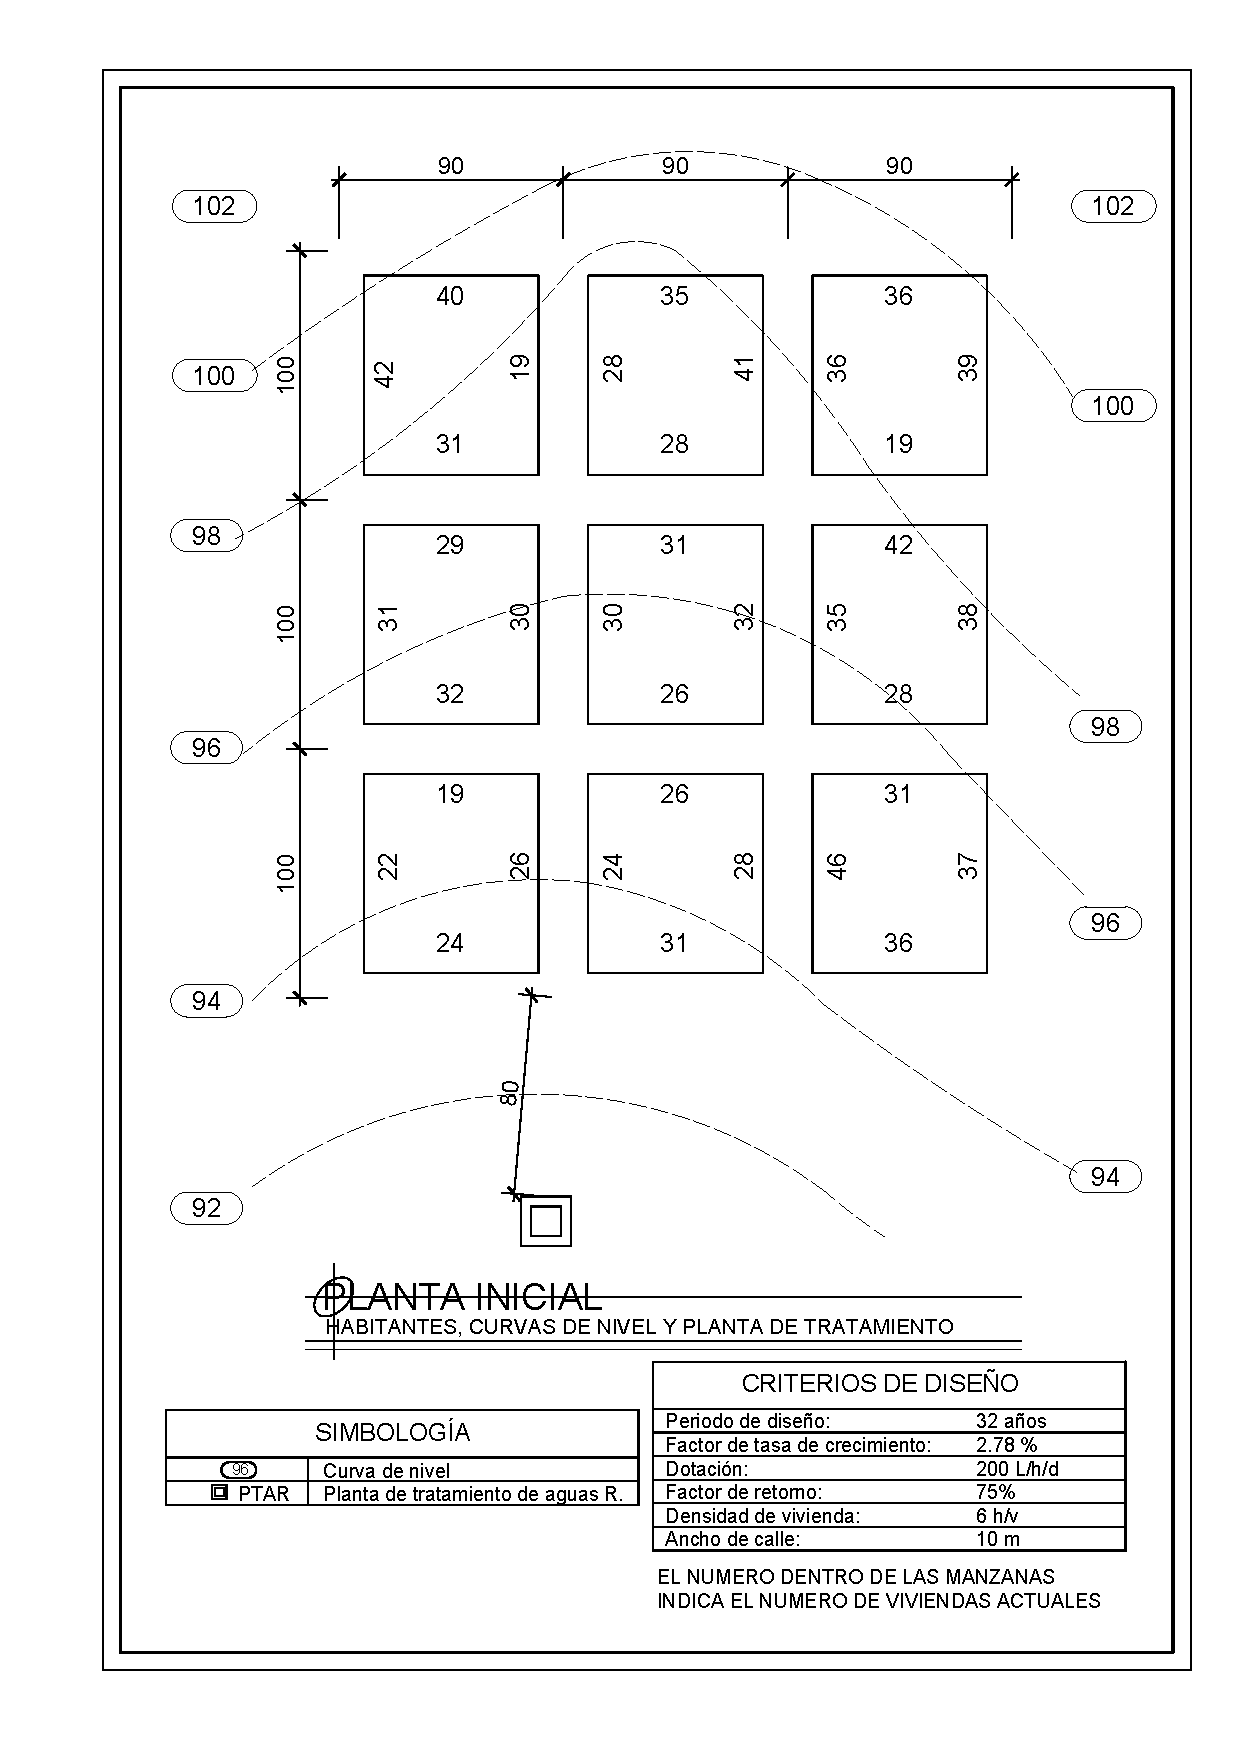
\includepdf[pages=-, pagecommand={}, fitpaper=true]{planodrenaje}
	

	

	
	\begin{figure}[H]\centering
		
\includegraphics[width=0.5\textwidth]{img4}
		\caption{Ancho de calle considerado.}\label{fig:img4}
	\end{figure}
	
	\begin{figure}[H]\centering
		
\includegraphics[width=0.5\textwidth]{img5}
		\caption{puntos de desfogue}\label{fig:img5}
	\end{figure}
	
	\begin{figure}[H]\centering
		
\includegraphics[width=0.5\textwidth]{img6}
		\caption{Criterios de diseño, drenaje}\label{fig:img6}
	\end{figure}
	
	\begin{figure}[H]\centering
		
\includegraphics[width=0.5\textwidth]{img7}
		\caption{Información de Pozos}\label{fig:img7}
	\end{figure}
	
	\begin{figure}[H]\centering
		
\includegraphics[width=1\textwidth]{img8}
		\caption{Diseño de Caudales}\label{fig:img8}
	\end{figure}
	
	
\subsection{Juntas en pavimento rígido y compactación del concreto}

\subsubsection{Juntas en pavimento rígido}
En los \textbf{pavimentos de concreto hidráulico}, las juntas son cortes o separaciones diseñadas para controlar los esfuerzos de contracción y expansión, y evitar fisuras aleatorias. Su función principal es permitir los movimientos del concreto por temperatura y humedad, y asegurar una transferencia adecuada de carga entre losas contiguas.

Los tipos más comunes son:
\begin{itemize}
	\item \textbf{Juntas de contracción:} inducen la fisura en un punto controlado al reducir la sección efectiva de la losa. Generalmente se cortan a una profundidad de 1/4 a 1/3 del espesor total de la losa.
	\item \textbf{Juntas de construcción:} se colocan donde se interrumpe el colado. Deben incluir pasadores o barras de amarre para mantener la continuidad estructural.
	\item \textbf{Juntas longitudinales:} separan los carriles adyacentes y controlan las fisuras por alabeo o contracción. Se utilizan barras de amarre para evitar la separación entre losas.
	\item \textbf{Juntas de expansión:} permiten el libre movimiento de las losas frente a estructuras fijas o cambios térmicos. Contienen materiales compresibles y se sellan para evitar el ingreso de agua.
\end{itemize}

El espaciamiento entre juntas de contracción suele variar entre 4 y 6 metros, dependiendo del espesor de la losa, las condiciones térmicas y el tipo de tráfico. Las juntas se sellan con materiales flexibles para impedir la filtración de agua y la entrada de partículas que puedan generar deterioro.

\subsubsection{Compactación del pavimento rígido}
La \textbf{compactación} en pavimentos rígidos comprende dos etapas: la compactación del suelo de apoyo y la consolidación del concreto fresco.

\paragraph{a) Compactación de subrasante y base:}
Antes del colado del concreto, el terreno debe alcanzar una \textit{densidad mínima del 95\% de la densidad seca máxima} obtenida en el ensayo Proctor modificado. Esto garantiza un soporte uniforme y reduce asentamientos diferenciales. La verificación se realiza mediante los métodos del \textit{cono de arena}, \textit{balón de caucho} o \textit{densímetro nuclear}.  

La densidad seca en campo se calcula con:
\[
\rho_d = \frac{\rho_h}{1+w}
\]
y el grado de compactación:
\[
GC(\%) = \frac{\rho_{d,\text{campo}}}{\rho_{d,\text{máx}}} \times 100
\]

\paragraph{b) Consolidación del concreto:}
El concreto fresco no se compacta en el sentido tradicional, sino que se \textbf{consolida} mediante vibración interna o superficial para eliminar burbujas de aire y asegurar contacto entre el concreto, el acero de refuerzo y la base. Una vibración adecuada mejora la resistencia, la durabilidad y la apariencia del pavimento. Es importante evitar la \textit{sobrevibración}, que puede causar segregación o exudación excesiva.

\subsubsection{Importancia de las juntas y la compactación}
Las juntas y la correcta compactación son fundamentales para garantizar la durabilidad del pavimento rígido. Las juntas controlan las grietas y permiten los movimientos del material, mientras que la compactación y consolidación aseguran una estructura estable y uniforme. El incumplimiento de estas prácticas puede provocar fisuración prematura, bombeo, asentamientos y fallas estructurales en el pavimento.

	
	
	\subsection{Ensayos de Compactación y Determinación de Densidad en Campo}
	
	\subsubsection{Ensayo CBR (California Bearing Ratio)}
	
	El \textbf{CBR} o \textit{California Bearing Ratio} es un ensayo que permite determinar la resistencia al esfuerzo cortante de un suelo, expresada como un porcentaje de la resistencia de un material patrón (generalmente piedra triturada bien graduada). Este ensayo fue desarrollado por el Departamento de Transporte de California y es ampliamente utilizado en ingeniería vial para evaluar la capacidad de soporte del suelo en el diseño de pavimentos.
	
	El principio del método consiste en medir la presión necesaria para hacer penetrar un pistón estándar en una muestra de suelo compactado a una velocidad constante. El resultado se expresa como un porcentaje de la presión que se requeriría para penetrar el mismo pistón en un material patrón. Matemáticamente se representa como:
	
	\[
	CBR = \frac{P_s}{P_p} \times 100
	\]
	
	donde:
	\begin{itemize}
		\item \( P_s \) = carga unitaria aplicada al suelo (kg/cm\(^2\))
		\item \( P_p \) = carga unitaria aplicada al material patrón (kg/cm\(^2\))
	\end{itemize}
	
	El valor de CBR se obtiene generalmente a dos penetraciones: 2.5 mm y 5.0 mm, tomando la mayor como resultado final. Los valores típicos varían entre 2\% (suelos muy blandos) hasta más de 80\% (materiales granulares bien compactados). Este parámetro es esencial para determinar el espesor de las capas estructurales en carreteras, calles y caminos rurales.
	
	\vspace{0.5cm}
	
	\subsubsection{Ensayo Proctor}
	
	El \textbf{ensayo Proctor} tiene como objetivo determinar la \textit{relación entre el contenido de humedad y la densidad seca} de un suelo, para una energía de compactación determinada. Existen dos versiones principales:
	\begin{itemize}
		\item \textbf{Proctor estándar (ASTM D698)}: se utiliza para suelos de baja o mediana plasticidad y energías de compactación moderadas.
		\item \textbf{Proctor modificado (ASTM D1557)}: aplica una energía mayor, representando condiciones de compactación más exigentes como las que se emplean en carreteras o aeropistas.
	\end{itemize}
	
	Durante el ensayo, se compacta el suelo en un molde cilíndrico en varias capas con un número determinado de golpes de un pisón metálico. Para cada muestra con diferente contenido de humedad, se determina la densidad seca correspondiente. Posteriormente, se grafica la curva de compactación (densidad seca vs. humedad), a partir de la cual se obtiene:
	\begin{itemize}
	
		\item \textbf{Humedad óptima (\( w_{opt} \))}, que es el contenido de humedad que permite alcanzar dicha densidad máxima.
	\end{itemize}
	
	Estos parámetros se utilizan como referencia para el control de compactación en campo, garantizando que los suelos alcancen condiciones adecuadas de soporte.
	
	\vspace{0.5cm}
	
	\subsubsection{Relación entre el Ensayo CBR y el Proctor}
	
	El ensayo \textbf{Proctor} proporciona la información necesaria para la preparación de las muestras del ensayo \textbf{CBR}. Es decir, el valor de densidad seca máxima y humedad óptima obtenidos en el Proctor se utilizan como parámetros de referencia para compactar las probetas del CBR antes de someterlas al ensayo de penetración.
	
	Por lo tanto, existe una relación directa: el CBR depende de la densidad y humedad con las que se compactó el suelo. En general, a mayor densidad (mayor grado de compactación), mayor será el valor del CBR. De igual forma, una humedad superior o inferior a la óptima puede reducir la resistencia del suelo. Esto demuestra la importancia de realizar ambos ensayos en conjunto para el diseño y control de calidad de capas estructurales en pavimentos.
	
	\vspace{0.5cm}
	
	\subsubsection{Determinación de la Densidad y Humedad en Campo}
	
	La densidad y el contenido de humedad en campo se determinan con el objetivo de comparar los resultados obtenidos con los valores de laboratorio (Proctor) y verificar que la compactación cumpla con el grado especificado (por ejemplo, 95\% de la densidad seca máxima).
	
	Existen varios métodos para determinar la densidad en campo:
	
	\begin{enumerate}
		\item \textbf{Método del cono de arena (ASTM D1556)}: consiste en excavar un pequeño hueco en el terreno, pesar el material extraído y llenar el hueco con arena calibrada. La relación entre el peso y volumen de arena desplazada permite calcular el volumen del hueco, y por tanto, la densidad húmeda del suelo.
		\item \textbf{Método del balón de caucho (ASTM D2167)}: se utiliza un dispositivo con un balón de goma lleno de agua, que se expande dentro del hueco excavado. El volumen desplazado se mide por el cambio de nivel de agua.
		\item \textbf{Método del densímetro nuclear (ASTM D6938)}: mide simultáneamente la densidad húmeda y el contenido de humedad mediante radiación gamma y neutrones. Es un método rápido y de alta precisión.
	\end{enumerate}
	
	Para determinar el \textbf{contenido de humedad}, se toma una muestra representativa del suelo y se seca en horno a 105–110°C durante 24 horas, siguiendo la norma ASTM D2216. La humedad se calcula con la expresión:
	
	\[
	w = \frac{(W_h - W_s)}{W_s} \times 100
	\]
	
	donde:
	\begin{itemize}
		\item \( W_h \) = peso del suelo húmedo (g)
		\item \( W_s \) = peso del suelo seco (g)
	\end{itemize}
	
	Finalmente, la \textbf{densidad seca en campo} se obtiene aplicando la relación:
	
	\[
	\rho_d = \frac{\rho_h}{1 + w}
	\]
	
	donde \( \rho_h \) es la densidad húmeda y \( w \) el contenido de humedad (en fracción decimal). Comparando este valor con la densidad seca máxima del Proctor se puede establecer el grado de compactación del terreno:
	

	
	\[
	\text{Grado de compactación (\%)} \;=\;
	\frac{\rho_{d,\text{campo}}}{\rho_{d,\text{máx}}}\times 100
	\]
	
	
	Este parámetro es esencial para el control de calidad de las obras de movimiento de tierras, rellenos estructurales y pavimentos.
	
	
	
	
	
	\section{Conclusiones}
	
	\textbf{Respecto al objetivo general:} \\
	Durante el desarrollo de las prácticas profesionales en la empresa \textit{Construcción e Ingeniería S.A.}, se logró aplicar de manera integral los conocimientos adquiridos en la carrera de Ingeniería Civil, especialmente en el área de topografía. A través de la ejecución de levantamientos, replanteos y control de niveles en proyectos reales —como el levantamiento de pozos, el trazado de tuberías, la verificación de rasantes y la alineación de bordillos— se fortalecieron las competencias técnicas y profesionales, contribuyendo al aseguramiento de la calidad y precisión geométrica de las obras ejecutadas en el Residencial Ceres III, Chichigüitán, Quetzaltenango.
	
	\vspace{0.3cm}
	\textbf{Respecto al primer objetivo específico:} \\
	Se ejecutaron y apoyaron levantamientos topográficos con el uso de estación total y niveles automáticos, lo que permitió obtener datos precisos de altitud, alineación y pendientes. Estos datos fueron esenciales para el correcto establecimiento de puntos de referencia en campo y para la posterior ejecución de trabajos de excavación y colocación de tuberías, garantizando la exactitud de los diseños proyectados.
	
	\vspace{0.3cm}
	\textbf{Respecto al segundo objetivo específico:} \\
	Durante la práctica se participó activamente en el trazado y control de obras civiles, verificando cotas y pendientes en la instalación de tuberías, pozos y secciones viales. Las actividades incluyeron el control geométrico de cruces de tubería bajo calzada, replanteo de tanques de captación y bordillos, así como el control de juntas de corte en pavimento. Gracias a estas verificaciones se logró mantener la precisión de los procesos constructivos y la uniformidad geométrica del proyecto.
	
	\vspace{0.3cm}
	\textbf{Respecto al tercer objetivo específico:} \\
	Se analizaron e interpretaron planos topográficos y constructivos, comparando los datos proyectados con las condiciones reales del sitio. Esto permitió realizar ajustes de rasante, corregir alineaciones y definir cotas de corte y relleno, asegurando la correspondencia entre el diseño y la realidad en campo. Dicho análisis facilitó la toma de decisiones oportunas y técnicas para la correcta ejecución de cada etapa de obra.
	
	\vspace{0.3cm}
	\textbf{Respecto al cuarto objetivo específico:} \\
	Se colaboró en la elaboración de informes y planos topográficos digitales, integrando información de campo mediante software especializado (\textit{AutoCAD}, \textit{Excel} y \textit{Civil 3D}). Esta labor permitió documentar de forma técnica las actividades desarrolladas, elaborar reportes de avance y cuantificación de áreas y volúmenes, y fortalecer las habilidades en el manejo de herramientas tecnológicas aplicadas al control y supervisión de proyectos de ingeniería civil.
	
	
	
	
	
	
	

	
	\section{Recomendaciones}
	
	\begin{enumerate}
		\item Seria bueno que se tuviera un contacto o un acercamiento antes a obras de construcción como  supervisión, control de materiales y seguimiento de avances etc, así también mas practicas de topografía en los cursos de la Universidad
		\item Considerar previamente reglamentos municipales y otros reglamentos necesarios para los conocimientos de rasantes y pendientes hidráulicas. 
		\item Considerar tener un manual tecnico sobre  levantamientos de control, resecciones, control geométrico de tuberías, verificación de sub-base/base y ejecución de juntas. 
		\item Incorporar conocimientos practicos sobre los siguientes software como  \textit{AutoCAD}/\textit{Civil 3D} y hojas de \textit{Excel}  \textit{QGIS}/\textit{ArcGIS} ya que son muy importantes para elementos y aplicaciones sobre informes  que pide la empresa 
		\item Prever las medidas de calidad, seguridad y cuidado del ambiente, en las distintas empresas donde se ejecute cualquier proyecto 
		
	\end{enumerate}
	
	
	
	
	\begin{thebibliography}{99}
		
		
		
		\bibitem{Lopez2019}
		López Hernández, J. A. (2019). \textit{Topografía aplicada a la ingeniería civil}. Bogotá, Colombia: Ecoe Ediciones.
		
		\bibitem{Gomez2017}
		Gómez Ramos, R. (2017). \textit{Manual de levantamientos topográficos y control de obras civiles}. Ciudad de México: Trillas.
		
		\bibitem{Perez2021}
		Pérez Martínez, L. F. (2021). \textit{Evaluación topográfica para el control geométrico en obras de urbanización}. (Tesis de grado). Universidad de San Carlos de Guatemala, Centro Universitario de Occidente (CUNOC).
		
		\bibitem{Martinez2020}
		Martínez López, D. R. (2020). \textit{Análisis del proceso de compactación y control de calidad en pavimentos de concreto hidráulico}. (Tesis de grado). Universidad Rafael Landívar, Guatemala.
		
		\bibitem{Rodriguez2022}
		Rodríguez, C. E. (2022). \textit{Uso de estación total en levantamientos y replanteos para proyectos de urbanización}. (Tesis de grado). Universidad de San Carlos de Guatemala, Facultad de Ingeniería.
		
		\bibitem{MOP2020}
		Ministerio de Comunicaciones, Infraestructura y Vivienda – MIVI. (2020). \textit{Guía técnica para obras viales y de drenaje en zonas urbanas}. Guatemala: Dirección General de Caminos.
		
		\bibitem{Sotelo2021}
		Sotelo, E. F. (2021). \textit{Control geométrico de obras civiles: teoría y práctica}. Madrid: Ediciones Díaz de Santos.
		
		\bibitem{INE2022}
		Instituto Nacional de Estadística (INE). (2022). \textit{Anuario estadístico de la construcción en Guatemala}. Guatemala: INE.
		
	\end{thebibliography}
	
	
	\section{Anexos}
	
	
\includepdf[pages=-, pagecommand={}, fitpaper=true]{investigacion2}
	
	
\end{document}

